\PassOptionsToPackage{unicode=true}{hyperref} % options for packages loaded elsewhere
\PassOptionsToPackage{hyphens}{url}
%
\documentclass[12pt,12pt,openright,oneside,a4paper,chapter=TITLE,section=TITLE,subsection=TITLE,subsubsection=TITLE,english,french,spanish,portugues,sumario=tradicional]{abntex2}
\usepackage{lmodern}
\usepackage{amssymb,amsmath}
\usepackage{ifxetex,ifluatex}
\usepackage{fixltx2e} % provides \textsubscript
\ifnum 0\ifxetex 1\fi\ifluatex 1\fi=0 % if pdftex
  \usepackage[T1]{fontenc}
  \usepackage[utf8]{inputenc}
  \usepackage{textcomp} % provides euro and other symbols
\else % if luatex or xelatex
  \usepackage{unicode-math}
  \defaultfontfeatures{Ligatures=TeX,Scale=MatchLowercase}
\fi
% use upquote if available, for straight quotes in verbatim environments
\IfFileExists{upquote.sty}{\usepackage{upquote}}{}
% use microtype if available
\IfFileExists{microtype.sty}{%
\usepackage[]{microtype}
\UseMicrotypeSet[protrusion]{basicmath} % disable protrusion for tt fonts
}{}
\IfFileExists{parskip.sty}{%
\usepackage{parskip}
}{% else
\setlength{\parindent}{0pt}
\setlength{\parskip}{6pt plus 2pt minus 1pt}
}
\usepackage{hyperref}
\hypersetup{
            pdfauthor={Jackson da Silva Torres},
            pdfborder={0 0 0},
            breaklinks=true}
\urlstyle{same}  % don't use monospace font for urls
\usepackage{longtable,booktabs}
% Fix footnotes in tables (requires footnote package)
\IfFileExists{footnote.sty}{\usepackage{footnote}\makesavenoteenv{longtable}}{}
\usepackage{graphicx,grffile}
\makeatletter
\def\maxwidth{\ifdim\Gin@nat@width>\linewidth\linewidth\else\Gin@nat@width\fi}
\def\maxheight{\ifdim\Gin@nat@height>\textheight\textheight\else\Gin@nat@height\fi}
\makeatother
% Scale images if necessary, so that they will not overflow the page
% margins by default, and it is still possible to overwrite the defaults
% using explicit options in \includegraphics[width, height, ...]{}
\setkeys{Gin}{width=\maxwidth,height=\maxheight,keepaspectratio}
\setlength{\emergencystretch}{3em}  % prevent overfull lines
\providecommand{\tightlist}{%
  \setlength{\itemsep}{0pt}\setlength{\parskip}{0pt}}
\setcounter{secnumdepth}{5}
% Redefines (sub)paragraphs to behave more like sections
\ifx\paragraph\undefined\else
\let\oldparagraph\paragraph
\renewcommand{\paragraph}[1]{\oldparagraph{#1}\mbox{}}
\fi
\ifx\subparagraph\undefined\else
\let\oldsubparagraph\subparagraph
\renewcommand{\subparagraph}[1]{\oldsubparagraph{#1}\mbox{}}
\fi

% set default figure placement to htbp
\makeatletter
\def\fps@figure{htbp}
\makeatother

%\usepackage{geometry}


% Pacotes básicos 
% ----------------------------------------------------------
%\usepackage{lmodern}			% Usa a fonte Latin Modern			
\usepackage[utf8]{inputenc}		% Codificacao do documento (conversão automática dos acentos)
\usepackage{csquotes}
\usepackage[T1]{fontenc}		% Selecao de codigos de fonte.
\usepackage{lastpage}			% Usado pela Ficha catalográfica
\usepackage{indentfirst}		% Indenta o primeiro parágrafo de cada seção.
\usepackage{color}		    	% Controle das cores
\usepackage{graphicx}			% Inclusão de gráficos
\usepackage{microtype} 			% para melhorias de justificação
\usepackage{ifthen}		    	% para montar condicionais
%\usepackage[brazil]{babel}		% para utilizar termos em portugues
\usepackage[final]{pdfpages}    % para incluir páginas de arquivos pdf
\usepackage{lipsum}				% para geração de dummy text
\usepackage{csquotes}

%\usepackage[style=long]{glossaries}
%\usepackage{abntex2glossaries}

% permite representar o cancelamento de termos em texto ou equacoes
\usepackage{cancel} 		
% cores extendidas
\usepackage{xcolor} 		
% gera diagramas a partir de listas
\usepackage{smartdiagram}   
% Para a figura ficar na posição correta
\usepackage{float} 		    
% supporte para fontes da Text Companion 
\usepackage{textcomp} 		
% uso de longtable
\usepackage{longtable}		
% simbolos matematicos
\usepackage{amsmath}	
% páginas em paisagem
\usepackage{lscape}
% mescla de colunas em tabelas
\usepackage{multicol}
% mescla de linhas em tabelas
\usepackage{multirow}
% criação do indice de quadros
\usepackage{newfloat} 
% configura legenda 
\usepackage{caption} 		
%[format=plain]
	%\renewcommand\caption[1]{%
    \captionsetup{font=small}	% tamanho da fonte 10pt
    %,format=hang
 	% \caption{#1}}
	%\captionsetup{width=0.8\textwidth}
	
%\usepackage{scrpage2}

% Pacotes de citações BibLaTeX
% ----------------------------------------------------------
\usepackage[
style=abnt,
%backref=true,
backend=biber,
maxcitenames=3,
%citecounter=true,
%backrefstyle=three,
nohashothers=true
]{biblatex}


\DefineBibliographyStrings{brazil}{%
 backrefpage = {Citado \arabic{citecounter} vez na página},% originally "cited on page"
 backrefpages = {Citado \arabic{citecounter} vezes nas páginas},% originally "cited on pages"
}

% ----------------------------------------------------------

% alterando o aspecto da cor azul
\definecolor{blue}{RGB}{55,10,249}

% ----------------------------------------------------------
\PrepareListOf{quadro}{%
\renewcommand{\cftfigpresnum}{Quadro~}}

\DeclareFloatingEnvironment[
fileext=loq,
listname={\textbf{LISTA DE QUADROS}},
name=Quadro,
%placement=p,
within= none, % numeracao continua
%within=section, % numeracao reinicia em cada seccao
%chapterlistsgaps=off
]{quadro}

\newlistentry{quadro}{loq}{0}


% Customize ‘List of Diagrams’
\PrepareListOf{quadro}{%
\renewcommand{\cftquadropresnum}{\normalsize{QUADRO}~}
\setlength{\cftquadronumwidth}{3.2cm}
%\renewcommand{\cftquadroname}{\quadroname\space} 
\renewcommand*{\cftquadroaftersnum}{\hfill--\hfill}
}

\makeatletter
%% we define a helper macro for adjusting lists of new floats to
%% accept a * behind them for not being shown in the TOC, like
%% the other list printing commands in memoir
\newcommand{\AdjustForMemoir}[1]{%
  \csletcs{kept@listof#1}{listof#1}%
  \csdef{listof#1}{%
    \@ifstar
     {\csappto{newfloat@listof#1@hook}{\append@star}%
      \csuse{kept@listof#1}}%
     {\csuse{kept@listof#1}}%
  }
}
\def\append@star#1{#1*}
\makeatother


\AdjustForMemoir{quadro} % prepare `\listofdirfigures` so it accepts a *

\makeatletter
\let\oldcontentsline\contentsline
\def\contentsline#1#2{%
    \expandafter\ifx\csname l@#1\endcsname\l@section
	\expandafter\@firstoftwo
	\else
	\expandafter\@secondoftwo
	\fi
	{%
		\oldcontentsline{#1}{\MakeTextUppercase{#2}}%
	}{%
	\normalsize %ajusta tamanho da fonte na lista
	\oldcontentsline{#1}{#2}%
}%
}
\makeatother

% Ajusta indentação de Referencias no ToC
% ----------------------------------------------------------
\defbibheading{bay}[\bibname]{%
  \chapter*{#1}%
  \markboth{#1}{#1}%
  \addcontentsline{toc}{chapter}
  {\protect\numberline{}\bibname}
}

\makeatletter
\pretocmd{\chapter}{\addtocontents{toc}{\protect\addvspace{-5\p@}}}{}{}
\pretocmd{\section}{\addtocontents{toc}{\protect\addvspace{2\p@}}}{}{}
\makeatother



%%%%%%%%%%%%%%% ALTERADO

% para citar tabelas e figuras no texto
\usepackage{hyperref}
\usepackage{varioref}

%%% auxiliar para kable

\usepackage{booktabs}
\usepackage{longtable}
\usepackage{array}
\usepackage{multirow}
\usepackage{wrapfig}
\usepackage{float}
\usepackage{colortbl}
\usepackage{pdflscape}
\usepackage{tabu}
\usepackage{threeparttable}
\usepackage{threeparttablex}
\usepackage[normalem]{ulem}
\usepackage{makecell}


%%%%%%%% Parágrafo

%\usepackage{fancyhdr}

%\usepackage{subcaption}
%\usepackage{booktabs}


%%%%%%% ESPAÇAMENTO 

%\usepackage{setspace}


%%%%%%%%%%%%%%%%%%%%%%%%%%%%%%%%%%%%%%%%%%%%%%%%%%%%%%%
% Arquivo para entrada de dados para a parte pré textual
%%%%%%%%%%%%%%%%%%%%%%%%%%%%%%%%%%%%%%%%%%%%%%%%%%%%%%%
% 
% Basta digitar as informações indicidas, no formato 
% apresentado.
%
%%%%%%%
% Os dados solicitados são, na ordem:
%
% tipo do trabalho
% componentes do trabalho 
% título do trabalho
% nome do autor
% local 
% data (ano com 4 dígitos)
% orientador(a)
% coorientador(a)(as)(es)
% arquivo com dados bibliográficos
% instituição
% setor
% programa de pós gradução
% curso
% preambulo
% data defesa
% CDU
% errata
% assinaturas - termo de aprovação
% resumos & palavras chave
% agradecimentos
% dedicatoria
% epígrafe


% Informações de dados para CAPA e FOLHA DE ROSTO
%----------------------------------------------------------------------------- 
\tipotrabalho{Dissertação}

% Marcar Sim para as partes que irão compor o documento pdf
%----------------------------------------------------------------------------- 
 \providecommand{\terCapa}{Sim}
 \providecommand{\terFolhaRosto}{Sim}
 \providecommand{\terTermoAprovacao}{Nao}
 \providecommand{\terDedicatoria}{Nao}
 \providecommand{\terFichaCatalografica}{Nao}
 \providecommand{\terEpigrafe}{Nao}
 \providecommand{\terAgradecimentos}{Nao}
 \providecommand{\terErrata}{Nao}
 \providecommand{\terListaFiguras}{Sim}
 \providecommand{\terListaTabelas}{Sim}
 \providecommand{\terSiglasAbrev}{Nao}
 \providecommand{\terResumos}{Nao}
 \providecommand{\terSumario}{Sim}
 \providecommand{\terAnexo}{Nao}
 \providecommand{\terApendice}{Nao}
 \providecommand{\terIndiceR}{Nao}
%----------------------------------------------------------------------------- 

\titulo{Efeitos das variações dos componentes do \emph{Spread} na rentabilidade das instituições bancárias através da análise de dados em painel
}
\autor{}
\local{Curitiba}
\data{2020} %Apenas ano 4 dígitos

% Orientador ou Orientadora
\orientador{}
%Prof Emílio Eiji Kavamura, MSc}
\orientadora{
Prof\textordfeminine~Dra. Mayla Costa}
% Pode haver apenas uma orientadora ou um orientador
% Se houver os dois prevalece o feminino.

% Em termos de coorientação, podem haver até quatro neste modelo
% Sendo 2 mulhere e 2 homens.
% Coorientador ou Coorientadora
\coorientador{}%Prof Morgan Freeman, DSc}
\coorientadora{}

% Segundo Coorientador ou Segunda Coorientadora
\scoorientador{}
%Prof Jack Nicholson, DEng}
\scoorientadora{}
%Prof\textordfeminine~Ingrid Bergman, DEng}
% ----------------------------------------------------------
%\addbibresource{10-references/referencias.bib}
%\bibliography{10-references/referencias.bib}
% ----------------------------------------------------------
\instituicao{Universidade Federal do Paraná}

\def \ImprimirSetor{Departamento de Economia}%
%Setor de Tecnologia}

\def \ImprimirProgramaPos{Programa Profissional de Pós-Graduação em Economia}

\def \ImprimirCurso{Mestrado Profissional em Economia}

\preambulo{
Trabalho apresentado como requisito parcial para a obtenção do título de Mestre Profisisonal em Economia no curso de Mestrado Profissional em Economia pelo Departamento de Economia da Universidade Federal do Paraná}
%do grau de Bacharel em Expressão Gráfica no curso de Expressão Gráfica, Setor de Exatas da Universidade Federal do Paraná}

%----------------------------------------------------------------------------- 

\newcommand{\imprimirCurso}{}
%Programa de P\'os Gradua\c{c}\~ao em Engenharia da Constru\c{c}\~ao Civil}

\newcommand{\imprimirDataDefesa}{
31 de Dezembro de 2020}

\newcommand{\imprimircdu}{
02:141:005.7}

% ----------------------------------------------------------
\newcommand{\imprimirerrata}{

\vspace{\onelineskip}


\begin{table}[htb]
\center
\footnotesize
\begin{tabular}{|p{1.4cm}|p{1cm}|p{3cm}|p{3cm}|}
  \hline
   \textbf{Folha} & \textbf{Linha}  & \textbf{Onde se lê}  & \textbf{Leia-se}  \\
    \hline
    1 & 10 & auto-conclavo & autoconclavo\\
   \hline
\end{tabular}
\end{table}}

% Comandos de dados - Data da apresentação
\providecommand{\imprimirdataapresentacaoRotulo}{}
\providecommand{\imprimirdataapresentacao}{}
\newcommand{\dataapresentacao}[2][\dataapresentacaoname]{\renewcommand{\dataapresentacao}{#2}}

% Comandos de dados - Nome do Curso
\providecommand{\imprimirnomedocursoRotulo}{}
\providecommand{\imprimirnomedocurso}{}
\newcommand{\nomedocurso}[2][\nomedocursoname]
  {\renewcommand{\imprimirnomedocursoRotulo}{#1}
\renewcommand{\imprimirnomedocurso}{#2}}


% ----------------------------------------------------------
\newcommand{\AssinaAprovacao}{

\assinatura{%\textbf
   {Professora} \\ UFPR}
   \assinatura{%\textbf
   {Professora} \\ ENSEADE}
   \assinatura{%\textbf
   {Professora} \\ TIT}
   %\assinatura{%\textbf{Professor} \\ Convidado 4}
      
   \begin{center}
    \vspace*{0.5cm}
    %{\large\imprimirlocal}
    %\par
    %{\large\imprimirdata}
    \imprimirlocal, \imprimirDataDefesa.
    \vspace*{1cm}
  \end{center}
  }
  
% ----------------------------------------------------------
%\newcommand{\Errata}{%\color{blue}
%Elemento opcional da \textcite[4.2.1.2]{NBR14724:2011}. Exemplo:
%}

% ----------------------------------------------------------
\newcommand{\EpigrafeTexto}{%\color{blue}
\textit{Texto}
}

% ----------------------------------------------------------
\newcommand{\ResumoTexto}{%\color{blue}

}

\newcommand{\PalavraschaveTexto}{%\color{blue}
latex. abntex. editoração de texto.}

% ----------------------------------------------------------
\newcommand{\AbstractTexto}{%\color{blue}
This is the english abstract.
}
% ---
\newcommand{\KeywordsTexto}{%\color{blue}
latex. abntex. text editoration.
}

% ----------------------------------------------------------
\newcommand{\Resume}
{%\color{blue}
Il s'agit d'un résumé en français.
} 
% ---
\newcommand{\Motscles}
{%\color{blue}
 latex. abntex. publication de textes.
}

% ----------------------------------------------------------
\newcommand{\Resumen}
{%\color{blue}
Este es el resumen en español.
}
% ---
\newcommand{\Palabrasclave}
{%\color{blue}
latex. abntex. publicación de textos.
}

% ----------------------------------------------------------
\newcommand{\AgradecimentosTexto}{%\color{blue}

}

% ----------------------------------------------------------
\newcommand{\DedicatoriaTexto}{%\color{blue}
\textit{}
	}


\makeindex
\usepackage{helvet}
\renewcommand{\familydefault}{\sfdefault}
\DeclareUnicodeCharacter{0301}{******}
\DeclareUnicodeCharacter{0303}{******}
\DeclareUnicodeCharacter{0327}{******}
\usepackage{booktabs}
\usepackage{longtable}
\usepackage{array}
\usepackage{multirow}
\usepackage{wrapfig}
\usepackage{float}
\usepackage{colortbl}
\usepackage{pdflscape}
\usepackage{tabu}
\usepackage{threeparttable}
\usepackage{threeparttablex}
\usepackage[normalem]{ulem}
\usepackage{makecell}
\usepackage{xcolor}
\usepackage[]{biblatex}

\author{Jackson da Silva Torres}
\date{2021}

\begin{document}

\chapter{Apresentação e análise dos resultados}

Em análise preliminar no conjunto de dados, levando em consideração as variáveis calculadas percebeu-se que a fórmula para \emph{spread ex-post} apresentada por \textcite{dantas:2012} e \textcite{timotio:2018} não é adequada para avaliar o mercado bancário como um todo, diante o fato de haver diferenças operacionais e operação de múltiplas carteiras.

A \autoref{table.spread.a} mostra o resultado do cálculo do \emph{spread ex-post} conforme equação \textcolor{red}{xxxxxx}, levando em consideração as receitas de crédito, operações de crédito, custo de captação e depósitos totais, com resultados que não refletem todas as operações exercidas pelas instituições.

\begin{table}
\caption{Cálculo Spread Ex-post com base nas Receitas de operações de crédito}
\begingroup\fontsize{10}{12}\selectfont

\begin{tabu} to \linewidth {>{\raggedleft}X>{\raggedleft}X>{\raggedleft}X>{\raggedleft}X>{\raggedleft}X}
\toprule
year(DATA) & SPREAD & Tx.Aplicação & Tx.Captação & DATA\\
\midrule
\cellcolor{gray!6}{2011} & \cellcolor{gray!6}{1.7224447} & \cellcolor{gray!6}{6.126370} & \cellcolor{gray!6}{4.403925} & \cellcolor{gray!6}{2011}\\
2012 & 1.4256950 & 5.065581 & 3.639886 & 2012\\
\cellcolor{gray!6}{2013} & \cellcolor{gray!6}{0.9068716} & \cellcolor{gray!6}{4.553858} & \cellcolor{gray!6}{3.646986} & \cellcolor{gray!6}{2013}\\
2014 & -0.3469018 & 4.674218 & 5.021120 & 2014\\
\cellcolor{gray!6}{2015} & \cellcolor{gray!6}{-0.4112076} & \cellcolor{gray!6}{5.328828} & \cellcolor{gray!6}{5.740035} & \cellcolor{gray!6}{2015}\\
\addlinespace
2016 & -1.2718303 & 4.997764 & 6.269595 & 2016\\
\cellcolor{gray!6}{2017} & \cellcolor{gray!6}{-0.3032622} & \cellcolor{gray!6}{4.611052} & \cellcolor{gray!6}{4.914314} & \cellcolor{gray!6}{2017}\\
2018 & 1.2279495 & 4.343456 & 3.115506 & 2018\\
\cellcolor{gray!6}{2019} & \cellcolor{gray!6}{1.3502961} & \cellcolor{gray!6}{4.310835} & \cellcolor{gray!6}{2.960539} & \cellcolor{gray!6}{2019}\\
2020 & 2.1606633 & 3.691604 & 1.530941 & 2020\\
\bottomrule
\end{tabu}
\endgroup{}
\label{table.spread.a}
\fonte{Densenvolvido a partir dos dados coletados}
\end{table}

Diante esta observação foi realizado um cálculo para o \emph{spread ex-post}, de tal modo que captasse as diferenças entre modalidades bancárias e operações das instituições, levando em consideração todas as receitas operacionais e as operações de crédito e outros créditos chegando ao resultado médio anual demonstrado na \autoref{table.spread.b}.

\begin{table}
\caption{Cálculo Spread Ex-post com base nas Receitas de operações de créditoCálculo Spread Ex-post com base na operações totais}
\begingroup\fontsize{10}{12}\selectfont

\begin{tabu} to \linewidth {>{\raggedleft}X>{\raggedleft}X>{\raggedleft}X>{\raggedleft}X}
\toprule
DATA & SPREAD & Tx.Aplicação & Tx.Captação\\
\midrule
\cellcolor{gray!6}{2011} & \cellcolor{gray!6}{14.83930} & \cellcolor{gray!6}{19.24322} & \cellcolor{gray!6}{4.403925}\\
2012 & 12.78096 & 16.42084 & 3.639886\\
\cellcolor{gray!6}{2013} & \cellcolor{gray!6}{11.69613} & \cellcolor{gray!6}{15.34311} & \cellcolor{gray!6}{3.646986}\\
2014 & 11.10626 & 16.12738 & 5.021120\\
\cellcolor{gray!6}{2015} & \cellcolor{gray!6}{12.17626} & \cellcolor{gray!6}{17.91630} & \cellcolor{gray!6}{5.740035}\\
\addlinespace
2016 & 10.89771 & 17.16730 & 6.269595\\
\cellcolor{gray!6}{2017} & \cellcolor{gray!6}{11.89732} & \cellcolor{gray!6}{16.81164} & \cellcolor{gray!6}{4.914314}\\
2018 & 11.94695 & 15.06246 & 3.115506\\
\cellcolor{gray!6}{2019} & \cellcolor{gray!6}{13.46580} & \cellcolor{gray!6}{16.42634} & \cellcolor{gray!6}{2.960539}\\
2020 & 13.85701 & 15.38795 & 1.530941\\
\bottomrule
\end{tabu}
\endgroup{}
\label{table.spread.b}
\fonte{Densenvolvido a partir dos dados coletados}
\end{table}

\[
SprEp = \frac{RcOpCr}{\frac{1}{2} * OpTot_{t} + OpTot_{t-1}} - \frac{DesCap}{\frac{1}{2} * DepTot_{t} + DepTot_{t-1} }
\]

Outro aspecto em relação as informações contábeis é que a conta de operações de crédito (16000001) que já se apresenta reduzida do valor de provisão para operações de crédito (16900008), uma \emph{proxy} para a inadimplência para cada instituição, podendo levar a equívocos a utilização destas duas variáveis sem o tratamento adequados, para fins de estimação o valor da inadimplência foi inserido na operação de crédito e a inadimplência calculada como percentual deste valor.

O painel desenvolvido para a construção dos modelos resultou no total 11170 observações, 116 períodos de tempo, contemplando um total de 196 instituições flutuando a cada período, conforme \autoref{tb:rsumoobs}, caracterizando-se em um painel não balanceado.

\begin{table}
\caption{Resumo de dados do Painel}
\begingroup\fontsize{10}{12}\selectfont

\begin{tabu} to \linewidth {>{\raggedleft}X>{\raggedleft}X>{\raggedleft}X>{\raggedleft}X}
\toprule
TEMPO & OBSERVAÇÕES & INSTITUICÕES & VARIÁVEIS.EXPLICATIVAS\\
\midrule
\cellcolor{gray!6}{116} & \cellcolor{gray!6}{11170} & \cellcolor{gray!6}{196} & \cellcolor{gray!6}{19}\\
\bottomrule
\end{tabu}
\endgroup{}
\label{tb:rsumoobs}
\fonte{Densenvolvido a partir dos dados coletados}
\end{table}

Foi realizado o teste Dick-Fuller para checar a estacionariedade da série, indicando que é estacionária, conforme indicado na \autoref{tb:dickfuller} e visualizado no \autoref{graf:dickfuller}.

\begin{table}
\caption{Resultado do teste Dick-Fuller}
\vspace{-2mm}
\begingroup\fontsize{10}{12}\selectfont

\begin{tabu} to \linewidth {>{\raggedright}X>{\raggedright}X>{\raggedright}X>{\raggedright}X}
\toprule
ESTATÍSTICA & P.VALOR & PARÂMETROS & ALTERNATIVA\\
\midrule
\cellcolor{gray!6}{-12.052563219859} & \cellcolor{gray!6}{0.01} & \cellcolor{gray!6}{22} & \cellcolor{gray!6}{Estacionária}\\
\bottomrule
\end{tabu}
\endgroup{}
\vspace{1mm}
\label{tb:dickfuller}
\fonte{Desenvolvido a partir dos dados coletados}
\vspace{-2mm}
\end{table}

Foi realizada uma avaliação de correlação entre as variáveis do painel de dados, e conforme \autoref{graf:corr} foi detectada forte correlação entre algumas variáveis, o que viria a causar diversos problemas de estimação. Para contornar essa questão foram excluídas variáveis autocorrelacionadas que apresentavam similaridades teóricas ou sem significância.

\begin{grafico}[!htbp]
\vspace{20pt}
\caption{Correlação entre variáveis do painel}
\vspace{-7mm}

\begin{center}
\includegraphics{12-exportedfigures/chart.correlation-1} \end{center}
\vspace{-3mm}
\label{graf:corr}
\fonte{Desenvolvido a partir de dados coletados}
\vspace{-2mm}
\end{grafico}

Entre as variáveis que foram eliminadas estão a \emph{proxy} para capital próprio (\(EPr\)), participação de mercado (\(MkSh\)), grau de concentração (\(GrCon\)), operações de crédito total (\(OpCrTotal\)), \emph{spread ex-ante} (\(SprEa\)) e o Índice de preços ao consumidor (\(IPCA\)).

Foram eliminadas as variáveis \emph{dummy} de controle de capital (\(OCap\)) e caráter da instituição (\(CrIns\)), por falta de informações evolutivas. Somente a variável \emph{dummy} referente à taxonomia (\(TpIns\)) foi mantida no modelo, esperando que ela venha captar as diferenças operacionais.

O painel de dados foi modificado em algumas variáveis para se adequar a nova modelagem e evitar problemas de autocorrelação. Preliminarmente dos dados monetários foram escalonados para unidades em milhões. Para as variáves referentes a base monetária e meios de pagamentos foram aplicados o logarítimo natural e de forma alternativa para fins de ajustes, considerado a variacação no ao longo do tempo destas variáveis.

Foram incluídas no modelo as varíáveis de operações de crédito total (\(lnOpTot\)) e receita operacional total de cada instituição (\(lnROp\)), com aplicação de logarítimo natural. E para captar as diferenças operacionais foram incluídas as variáveis de participação das receitas segmentadas em relação as receitas operacionais: receitas de operação de crédito (\(ROpCr\)), receitas de serviços (\(RSrv\)), receitas de participações (\(RPart\)) e outras receitas operacionais (\(OtROp\))

Em relação a participação das modalidades de depósitos sobre as operações de créditos totais (\(OpCrTot\)), além dos dos depósitos a vista (\(DepAv\)) e depóstos a prazo (\(DepAp\)), foram incluídos os depósitos depoupança (\(DepPop\)), depositos interfinanceiros (\(DepIf\)) e outros depósitos (\(OtDep\)). Com objetivos de verificar o perfil de captação por modalidade e como este influencia no nível de \emph{spread}.

Para a inadimplência (\(Inad\)) passou-se a usar a participação da provisão para crédito duvidoso sobre a soma das operações de crédito e outros crédito (\(OpCrTot\))\footnote{Já adicionados dos próprios valores de provisão que se encontram subtraídos nas demonstrações contábeis}.

Para captar as diferenças no perfil de despesas por modalidadde de instituições e como este influencia no nível de \emph{spread} além das despesas administrativas em função das operações totais (\(DAdm\)) foram inclúídas as despesas de captação em função dos depósitos totais (\(DesCap\)) e outras despesas em função das operações de créditos totais (\(OtDes\)).

Finalizando os ajuste no modelo, foram incluídas as variáveis de impostos indiretos (\(ImpInd\)) e imposto de renda (\(ImpRen\)), completando as variáveis explícitas do \emph{spread}, com exceção do compulsório por apresentar forte correlação com outras variáveis e do do fundo garantidor de crédito por se demonstrar insignificante.

\begin{verbatim}
$$
\begin{aligned}
\operatorname{\widehat{SprEp}} &= 0.43 - 0.13(\operatorname{lnOpTot}) + 0.01(\operatorname{lnAtv}) + 0(\operatorname{DAdm})\ - \\
&\quad 0.67(\operatorname{DesCap}) + 0(\operatorname{OtDes}) + 0(\operatorname{Inad}) + 0(\operatorname{RcPd})\ + \\
&\quad 0(\operatorname{lnMPA4}) + 0.05(\operatorname{SelMet}) + 0(\operatorname{VelMo}) + 0(\operatorname{ImpRend})\ + \\
&\quad 0(\operatorname{ImpInd}) + 0(\operatorname{DepAv}) + 0(\operatorname{DepAp}) + 0(\operatorname{DepIf})\ + \\
&\quad 0(\operatorname{DepPop}) + 0.12(\operatorname{lnROp}) + 0.02(\operatorname{ROpCr}) + 0.04(\operatorname{RSrv})\ + \\
&\quad 0.06(\operatorname{RPart})
\end{aligned}
$$
\end{verbatim}

Os dados em painel foram estimados nos métodos \emph{pooling}, efeitos fixos e efeitos aleatórios com os resultados demonstrados na \autoref{tb:regress}, com coeficientes de determinação (\(R^2\)) 0.884, 0.883 e 0.849 respectivamente. A diferença entre as variáveis dos modelos está na adoção da variação dos meios de pagamento ampliados (\(M4\)) no modelo de efeitos aleatórios.

\begin{verbatim}
Pooling Model

Call:
plm(formula = SprEp ~ lnOpTot + lnAtv + lnROp + DAdm + DesCap + 
    OtDes + +Inad + RcPd + TpIns + SelMet + VelMo + ImpRend + 
    ImpInd + DepAv + DepAp + DepIf + DepPop + ROpCr + RSrv + 
    RPart, data = banksDf.model, model = "pooling", index = c("BANCO"))

Unbalanced Panel: n = 196, T = 1-116, N = 11170

Residuals:
     Min.   1st Qu.    Median   3rd Qu.      Max. 
-0.814190 -0.026316 -0.010039  0.019961  0.515258 

Coefficients:
                                  Estimate  Std. Error  t-value  Pr(>|t|)    
(Intercept)                     3.5416e-01  8.2689e-03  42.8296 < 2.2e-16 ***
lnOpTot                        -1.2718e-01  1.4397e-03 -88.3389 < 2.2e-16 ***
lnAtv                           1.0636e-02  9.6830e-04  10.9838 < 2.2e-16 ***
lnROp                           1.1701e-01  9.4825e-04 123.3967 < 2.2e-16 ***
DAdm                            4.6974e-07  1.7354e-08  27.0679 < 2.2e-16 ***
DesCap                         -6.7654e-01  9.5720e-03 -70.6796 < 2.2e-16 ***
OtDes                           9.0936e-07  1.1995e-08  75.8087 < 2.2e-16 ***
Inad                           -8.3059e-07  1.7348e-08 -47.8791 < 2.2e-16 ***
RcPd                           -2.8492e-04  1.6147e-04  -1.7646 0.0776554 .  
TpInsBANCOS COMERCIAIS          3.5557e-02  5.1449e-03   6.9111 5.072e-12 ***
TpInsBANCOS DE DESENVOLVIMENTO  3.9885e-02  6.0134e-03   6.6327 3.448e-11 ***
TpInsBANCOS DE INVESTIMENTO     4.2660e-02  5.4818e-03   7.7821 7.764e-15 ***
TpInsBANCOS MULTIPLOS           2.7886e-02  4.7632e-03   5.8544 4.923e-09 ***
TpInsBNDES                     -8.0212e-03  6.4232e-03  -1.2488 0.2117693    
TpInsCAIXA ECONOMICA FEDERAL   -5.0106e-03  6.3408e-03  -0.7902 0.4294160    
SelMet                          5.6561e-02  1.6175e-02   3.4969 0.0004725 ***
VelMo                           9.8186e-09  3.0003e-08   0.3273 0.7434814    
ImpRend                         1.4526e-08  1.6364e-09   8.8767 < 2.2e-16 ***
ImpInd                         -1.0548e-09  1.6686e-09  -0.6322 0.5272993    
DepAv                           8.4673e-09  3.3554e-09   2.5235 0.0116335 *  
DepAp                           9.5943e-09  8.6592e-10  11.0799 < 2.2e-16 ***
DepIf                           1.4931e-08  1.6608e-09   8.9904 < 2.2e-16 ***
DepPop                          5.2700e-08  5.5991e-09   9.4121 < 2.2e-16 ***
ROpCr                           2.7014e-02  2.5687e-03  10.5167 < 2.2e-16 ***
RSrv                            3.4078e-02  6.2452e-03   5.4567 4.954e-08 ***
RPart                           6.7284e-02  1.3214e-02   5.0918 3.605e-07 ***
---
Signif. codes:  0 '***' 0.001 '**' 0.01 '*' 0.05 '.' 0.1 ' ' 1

Total Sum of Squares:    218.97
Residual Sum of Squares: 25.013
R-Squared:      0.88577
Adj. R-Squared: 0.88551
F-statistic: 3456.56 on 25 and 11144 DF, p-value: < 2.22e-16
\end{verbatim}

\begin{verbatim}

Resultados das Regressões
================================================================================================
                                                      Dependent variable:                       
                               -----------------------------------------------------------------
                                                             SprEp                              
                                      Pooling            Efeitos Fixos      Efeitos Aleatórios  
                                        (1)                   (2)                   (3)         
------------------------------------------------------------------------------------------------
lnOpTot                          -0.127*** (0.001)     -0.117*** (0.002)     -0.121*** (0.002)  
                                    t = -88.339           t = -52.774           t = -64.844     
                                     p = 0.000             p = 0.000             p = 0.000      
lnAtv                            0.011*** (0.001)      0.006*** (0.002)      0.008*** (0.001)   
                                    t = 10.984             t = 3.452             t = 5.551      
                                     p = 0.000             p = 0.001            p = 0.00000     
lnROp                            0.117*** (0.001)      0.111*** (0.001)      0.113*** (0.001)   
                                    t = 123.397           t = 110.064           t = 114.128     
                                     p = 0.000             p = 0.000             p = 0.000      
DAdm                           0.00000*** (0.00000)  0.00000*** (0.00000)  0.00000*** (0.00000) 
                                    t = 27.068            t = 27.082            t = 26.905      
                                     p = 0.000             p = 0.000             p = 0.000      
DesCap                           -0.677*** (0.010)     -0.624*** (0.011)     -0.636*** (0.011)  
                                    t = -70.680           t = -55.588           t = -59.585     
                                     p = 0.000             p = 0.000             p = 0.000      
OtDes                           0.00000*** (0.000)    0.00000*** (0.000)    0.00000*** (0.000)  
                                    t = 75.809            t = 76.550            t = 76.972      
                                     p = 0.000             p = 0.000             p = 0.000      
Inad                           -0.00000*** (0.00000) -0.00000*** (0.00000) -0.00000*** (0.00000)
                                    t = -47.879           t = -46.733           t = -47.922     
                                     p = 0.000             p = 0.000             p = 0.000      
RcPd                             -0.0003* (0.0002)    -0.0004** (0.0002)    -0.0003** (0.0002)  
                                    t = -1.765            t = -2.470            t = -2.048      
                                     p = 0.078             p = 0.014             p = 0.041      
TpInsBANCOS COMERCIAIS           0.036*** (0.005)      0.014*** (0.005)       0.033* (0.019)    
                                     t = 6.911             t = 2.682             t = 1.727      
                                     p = 0.000             p = 0.008             p = 0.085      
TpInsBANCOS DE DESENVOLVIMENTO   0.040*** (0.006)                              0.030 (0.022)    
                                     t = 6.633                                   t = 1.358      
                                     p = 0.000                                   p = 0.175      
TpInsBANCOS DE INVESTIMENTO      0.043*** (0.005)        0.012 (0.024)        0.037* (0.020)    
                                     t = 7.782             t = 0.526             t = 1.877      
                                     p = 0.000             p = 0.599             p = 0.061      
TpInsBANCOS MULTIPLOS            0.028*** (0.005)                              0.021 (0.018)    
                                     t = 5.854                                   t = 1.125      
                                     p = 0.000                                   p = 0.261      
TpInsBNDES                        -0.008 (0.006)                              -0.009 (0.026)    
                                    t = -1.249                                  t = -0.348      
                                     p = 0.212                                   p = 0.729      
TpInsCAIXA ECONOMICA FEDERAL      -0.005 (0.006)                              -0.008 (0.025)    
                                    t = -0.790                                  t = -0.313      
                                     p = 0.430                                   p = 0.755      
SelMet                           0.057*** (0.016)      0.051*** (0.016)      0.049*** (0.016)   
                                     t = 3.497             t = 3.133             t = 3.069      
                                    p = 0.0005             p = 0.002             p = 0.003      
VelMo                             0.000 (0.00000)       0.000 (0.00000)       0.000 (0.00000)   
                                     t = 0.327             t = 0.216             t = 0.129      
                                     p = 0.744             p = 0.829             p = 0.898      
ImpRend                          0.000*** (0.000)      0.000*** (0.000)      0.000*** (0.000)   
                                     t = 8.877             t = 6.273             t = 6.797      
                                     p = 0.000             p = 0.000             p = 0.000      
ImpInd                            -0.000 (0.000)         0.000 (0.000)        -0.000 (0.000)    
                                    t = -0.632             t = 0.102            t = -0.131      
                                     p = 0.528             p = 0.919             p = 0.896      
DepAv                             0.000** (0.000)      -0.000*** (0.000)     -0.000** (0.000)   
                                     t = 2.523            t = -3.341            t = -2.380      
                                     p = 0.012             p = 0.001             p = 0.018      
DepAp                            0.000*** (0.000)      0.000*** (0.000)      0.000*** (0.000)   
                                    t = 11.080             t = 8.664             t = 8.014      
                                     p = 0.000             p = 0.000             p = 0.000      
DepIf                           0.00000*** (0.000)    0.00000*** (0.000)    0.00000*** (0.000)  
                                     t = 8.990             t = 9.006             t = 9.129      
                                     p = 0.000             p = 0.000             p = 0.000      
DepPop                          0.00000*** (0.000)    0.00000** (0.00000)  0.00000*** (0.00000) 
                                     t = 9.412             t = 2.541             t = 4.305      
                                     p = 0.000             p = 0.012            p = 0.00002     
ROpCr                            0.027*** (0.003)      0.022*** (0.004)      0.023*** (0.004)   
                                    t = 10.517             t = 5.348             t = 6.357      
                                     p = 0.000            p = 0.00000            p = 0.000      
RSrv                             0.034*** (0.006)       0.028** (0.012)      0.030*** (0.010)   
                                     t = 5.457             t = 2.320             t = 2.898      
                                    p = 0.00000            p = 0.021             p = 0.004      
RPart                            0.067*** (0.013)      0.055*** (0.017)      0.064*** (0.016)   
                                     t = 5.092             t = 3.197             t = 3.901      
                                    p = 0.00000            p = 0.002            p = 0.0001      
Constant                         0.354*** (0.008)                            0.360*** (0.021)   
                                    t = 42.830                                  t = 16.903      
                                     p = 0.000                                   p = 0.000      
------------------------------------------------------------------------------------------------
Observations                          11,170                11,170                11,170        
R2                                     0.886                 0.834                 0.851        
Adjusted R2                            0.886                 0.830                 0.851        
================================================================================================
Note:                                                                *p<0.1; **p<0.05; ***p<0.01
\end{verbatim}

Quitting from lines 934-935 (jacksontorres.Rmd)
Error in nchar(x) : invalid multibyte string, element 1
Calls: local \ldots{} split.large.cells -\textgreater{} sapply -\textgreater{} lapply -\textgreater{} FUN -\textgreater{} split.single.cell
In addition: There were 24 warnings (use warnings() to see them)

No modelo \emph{pooling}, não foi encontrada significância a 5\%, para as variáveis de meios de pagamentos (\(M4\)), velocidade da moeda (\(VelMo\)), impostos indiretos (\(ImpInd\)) e depositos a vista (\(DepAv\)). As demais variáveis apresentação elevado nível de significância. Foi aplicado o teste de Wooldridge aceitando a hipótese nula que os erros para a taxonomia não são relacionados.

\begin{table}
\caption{Resultado do teste Wooldridge para o modelo pooling}
\vspace{-2mm}

-----------------------------------------------------------
 Test statistic       P value       Alternative hypothesis 
---------------- ----------------- ------------------------
     5.664        1.479e-08 * * *     unobserved effect    
-----------------------------------------------------------

Table: Wooldridge's test for unobserved individual effects: `formula`
\vspace{1mm}
\label{tb:wdtest}
\fonte{Desenvolvido a partir dos dados estimados}
\vspace{-2mm}
\end{table}

Para comparação entre os modelos pooling e efeitos fixos foi aplicado o teste F de Chrow para avaliar os efeitos individuais, sendo rejeitada a hipótese nula de igualdade nos interceptos e coeficientes, indicando que o modelo de efeitos fixos seria mais adequado para estimação do modelo.

Para comparar os modelos pooling e efeitos aleatórios foi utilizado o teste Breusch-Pagan (multiplicador de lagrange) para modelos em painel não balanceados, rejeitando a hipótese nula que a variância dos erros são iguais, indicando heterocedasticidade, dando assim preferência ao modelo de efeitos aleatórios.

\begin{longtable}[]{@{}cccc@{}}
\caption{Lagrange Multiplier Test - (Breusch-Pagan) for unbalanced panels: \texttt{SprEp\ \textasciitilde{}\ lnOpTot\ +\ lnAtv\ +\ lnROp\ +\ DAdm\ +\ DesCap\ +\ OtDes\ +\ +Inad\ +\ \ ...}}\tabularnewline
\toprule
\begin{minipage}[b]{0.21\columnwidth}\centering
Test statistic\strut
\end{minipage} & \begin{minipage}[b]{0.06\columnwidth}\centering
df\strut
\end{minipage} & \begin{minipage}[b]{0.12\columnwidth}\centering
P value\strut
\end{minipage} & \begin{minipage}[b]{0.31\columnwidth}\centering
Alternative hypothesis\strut
\end{minipage}\tabularnewline
\midrule
\endfirsthead
\toprule
\begin{minipage}[b]{0.21\columnwidth}\centering
Test statistic\strut
\end{minipage} & \begin{minipage}[b]{0.06\columnwidth}\centering
df\strut
\end{minipage} & \begin{minipage}[b]{0.12\columnwidth}\centering
P value\strut
\end{minipage} & \begin{minipage}[b]{0.31\columnwidth}\centering
Alternative hypothesis\strut
\end{minipage}\tabularnewline
\midrule
\endhead
\begin{minipage}[t]{0.21\columnwidth}\centering
2781\strut
\end{minipage} & \begin{minipage}[t]{0.06\columnwidth}\centering
1\strut
\end{minipage} & \begin{minipage}[t]{0.12\columnwidth}\centering
0 * * *\strut
\end{minipage} & \begin{minipage}[t]{0.31\columnwidth}\centering
significant effects\strut
\end{minipage}\tabularnewline
\bottomrule
\end{longtable}

Em termos de comparação entre os modelos de efeitos fixos e efeitos aleatórios foi utilizado o teste de Hausman, com rejeição da hipotese nula (parâmetros não correlacionados), indicando assim correlação entre os parâmetros e indicando que o modelo e efeitos fixos é mais adequado para avaliação do modelo.

Para checar a dependência transversal do modelo de efeitos fixo foi utilizado o teste Pesaran, sendo rejeitada a hipótese nula (não correlação dos resíduos aos indivíduos) indicando que os resíduos entre os individuos estão correlacionados.

\begin{longtable}[]{@{}ccc@{}}
\caption{Pesaran CD test for cross-sectional dependence in panels: \texttt{SprEp\ \textasciitilde{}\ lnOpTot\ +\ lnAtv\ +\ +DAdm\ +\ DesCap\ +\ OtDes\ +\ +Inad\ +\ RcPd\ +\ \ \ \ \ TpIns\ +\ SelMet\ +\ VelMo\ +\ ImpRend\ +\ ImpInd\ +\ DepAv\ +\ DepAp\ +\ \ \ \ \ DepIf\ +\ DepPop\ +\ lnROp\ +\ ROpCr\ +\ RSrv\ +\ RPart}}\tabularnewline
\toprule
\begin{minipage}[b]{0.22\columnwidth}\centering
Test statistic\strut
\end{minipage} & \begin{minipage}[b]{0.23\columnwidth}\centering
P value\strut
\end{minipage} & \begin{minipage}[b]{0.37\columnwidth}\centering
Alternative hypothesis\strut
\end{minipage}\tabularnewline
\midrule
\endfirsthead
\toprule
\begin{minipage}[b]{0.22\columnwidth}\centering
Test statistic\strut
\end{minipage} & \begin{minipage}[b]{0.23\columnwidth}\centering
P value\strut
\end{minipage} & \begin{minipage}[b]{0.37\columnwidth}\centering
Alternative hypothesis\strut
\end{minipage}\tabularnewline
\midrule
\endhead
\begin{minipage}[t]{0.22\columnwidth}\centering
14.5\strut
\end{minipage} & \begin{minipage}[t]{0.23\columnwidth}\centering
1.214e-47 * * *\strut
\end{minipage} & \begin{minipage}[t]{0.37\columnwidth}\centering
cross-sectional dependence\strut
\end{minipage}\tabularnewline
\bottomrule
\end{longtable}

A normalidade dos resíduos do modelo de efeitos aletórios foi testado pelo método, rejeitando a hipótese nula de normalidade dos resíduos, indicando que o modelo apresenta problemas de hetetocedasticidadade.

\begin{longtable}[]{@{}ccc@{}}
\caption{studentized Breusch-Pagan test: \texttt{mod01.Pooling}}\tabularnewline
\toprule
\begin{minipage}[b]{0.22\columnwidth}\centering
Test statistic\strut
\end{minipage} & \begin{minipage}[b]{0.06\columnwidth}\centering
df\strut
\end{minipage} & \begin{minipage}[b]{0.13\columnwidth}\centering
P value\strut
\end{minipage}\tabularnewline
\midrule
\endfirsthead
\toprule
\begin{minipage}[b]{0.22\columnwidth}\centering
Test statistic\strut
\end{minipage} & \begin{minipage}[b]{0.06\columnwidth}\centering
df\strut
\end{minipage} & \begin{minipage}[b]{0.13\columnwidth}\centering
P value\strut
\end{minipage}\tabularnewline
\midrule
\endhead
\begin{minipage}[t]{0.22\columnwidth}\centering
2875\strut
\end{minipage} & \begin{minipage}[t]{0.06\columnwidth}\centering
25\strut
\end{minipage} & \begin{minipage}[t]{0.13\columnwidth}\centering
0 * * *\strut
\end{minipage}\tabularnewline
\bottomrule
\end{longtable}

Foi testada a correlação serial do modelo de efeitos fixos, rejeitando a hipotese nula (de não correlação serial), indicando assim que o painel de dados possui problemas de correlação serial entre dos dados.

\begin{longtable}[]{@{}cccc@{}}
\caption{Breusch-Godfrey/Wooldridge test for serial correlation in panel models: \texttt{SprEp\ \textasciitilde{}\ lnOpTot\ +\ lnAtv\ +\ +DAdm\ +\ DesCap\ +\ OtDes\ +\ +Inad\ +\ RcPd\ +\ \ \ \ \ TpIns\ +\ SelMet\ +\ VelMo\ +\ ImpRend\ +\ ImpInd\ +\ DepAv\ +\ DepAp\ +\ \ \ \ \ DepIf\ +\ DepPop\ +\ lnROp\ +\ ROpCr\ +\ RSrv\ +\ RPart}}\tabularnewline
\toprule
\begin{minipage}[b]{0.21\columnwidth}\centering
Test statistic\strut
\end{minipage} & \begin{minipage}[b]{0.06\columnwidth}\centering
df\strut
\end{minipage} & \begin{minipage}[b]{0.23\columnwidth}\centering
P value\strut
\end{minipage} & \begin{minipage}[b]{0.31\columnwidth}\centering
Alternative hypothesis\strut
\end{minipage}\tabularnewline
\midrule
\endfirsthead
\toprule
\begin{minipage}[b]{0.21\columnwidth}\centering
Test statistic\strut
\end{minipage} & \begin{minipage}[b]{0.06\columnwidth}\centering
df\strut
\end{minipage} & \begin{minipage}[b]{0.23\columnwidth}\centering
P value\strut
\end{minipage} & \begin{minipage}[b]{0.31\columnwidth}\centering
Alternative hypothesis\strut
\end{minipage}\tabularnewline
\midrule
\endhead
\begin{minipage}[t]{0.21\columnwidth}\centering
1106\strut
\end{minipage} & \begin{minipage}[t]{0.06\columnwidth}\centering
1\strut
\end{minipage} & \begin{minipage}[t]{0.23\columnwidth}\centering
1.991e-242 * * *\strut
\end{minipage} & \begin{minipage}[t]{0.31\columnwidth}\centering
serial correlation in
idiosyncratic errors\strut
\end{minipage}\tabularnewline
\bottomrule
\end{longtable}

Os resultados das estimações dos modelos, demonstrou elevada siginificância para as variáveis, com coeficientes de determinação acima dos 88\%, porém os testes indicaram problemas de heterocedasticidade e dependência cross-sectional, podendo estar inflando os resultados, demonstrando-se inadequados para uma estimação confiável.

Porém, de acordo com Sargan (1964) e Hendry e Mizon (1978), os testes de dependência cross-seccional não significam essencialmente que exista essa condição para o modelo, e sim um problema de especificação dinâmica, com a omissão de variáveis defasadas.

O modelo conceitual e economético desenvolvido está regido pelo dinamismo econômico, com uma variável dependente obtida através da diferença de dois termos de resultados, dependente de variáveis microecnômicas endógenas e de mercado, e de variáveis macroeconômicas, necessitando assim de uma modelagem que comporte esse dinamismo.

Diante as características do modelo, foi identificada a metodologia de painel de vetores autoregressivos (PVAR), que comporta mais de uma variável dependente defasadad, variáveis preditoras endógenas e variáveis preditoras exógenas com estimação por método de momentos generalizados (GMM) .

A metodologia PVAR mostra-se compatível com a característica de painel não balanceado (N \textgreater{} T), porém necessitando de tratamento em observações inciais, e enfretar problemas com a questão da heterogeneidade entre os grupos de cortes transversais. Tais limitações seriam contornadas com a utilização do método GMM (\uppercase{Newey e Rosen} 1988).

O modelo de estimar GMM proposto por Arellano e Bond (1991), vem contornar a incosistência dos modelos de efeitos fixos, utilizando variáveis defasadas como instrumentos para variáveis endógenas. O procedimento de estimação pode ser em uma etapa, ou duas etapas, onde esta se basea nos resíduos da primeira etapa. E uma matriz é utilizada para retirar o modelo de efeito fixo.

No modelo PVAR-GMM proposto por Arellano e Bond (1991) se alguma variável possuir raiz unitária, o estimador será inconsistente. Porém, de acordo com Binder, Hsiao e Pesaran (2005), seria mais eficiente do que estimar cada equação por GMM. Tal limitação seria contornada pela proposta de uma sistema GMM apresentado por Blundell e Bond (1998).

A proposta de Blundell e Bond (1998) consiste corrigir o viés causado pelos efeito fixos aplicados em painéis dinâmicos, através da modificação, ou seja, a retirada em primeira ordem, dos instrumentos, passando a serem exógenos aos efeitos fixos, assumindo que as variações nas variáveis instrumentais não são correlacionadas com os efeitos fixos e com o erro.

O novo painel foi desenvolvido com a eliminação de variáveis que ainda apresentavam nível de correlação considerado elevado para a metodologia. As variáveis de \emph{spread ex-post} (\(SprEp\)) e rentabilidade foram inseridas simultaneamente no modelo como depedentesntes, as variáveis micreconômicas foram inseridas como preditoras e as variáveis macroeconômicas foram inseridas como exógenas.

\textbackslash{}begin\{table\}{[}!hbtp{]}
\captionof{table}{Resultado do modelo PVAR-GMM}
\vspace{-2mm}

Dynamic Panel VAR estimation, one-step GMM

Transformation: Forward orthogonal deviationsGroup variable: BANCOTime variable: DATANumber of observations = 654Number of groups = 126Obs per group: min = 1Obs per group: avg = 7.03225806451613Obs per group: max = 9Number of instruments = 422

~

SprEp

Rent

lag1\_SprEp

0.0715**

-3.2560*

~

(0.0260)

(1.2784)

lag1\_Rent

-0.0051*

0.1488

~

(0.0021)

(0.1853)

lag2\_SprEp

-0.0437**

-0.6065

~

(0.0160)

(0.8242)

lag2\_Rent

-0.0031*

-0.0749

~

(0.0015)

(0.0695)

ImpRend

0.4411*

-16.8116*

~

(0.1770)

(8.5232)

ImpInd

-0.0844

2.7044*

~

(0.0464)

(1.0528)

EPr

0.0003

-0.0202

~

(0.0006)

(0.0134)

RcCr

-0.0919

-6.6041

~

(0.2346)

(11.0450)

DAdm

1.3201**

37.5553**

~

(0.4422)

(13.4838)

OtDes

2.7199***

2.8166

~

(0.2221)

(6.6387)

OpEmp

-0.5976

77.8192

~

(0.9681)

(53.2330)

OpFin

-0.1934

47.8021

~

(1.0013)

(50.6135)

OtOp

-0.3429

56.7566

~

(1.0118)

(53.6945)

ROpCr

0.0756

-2.5694

~

(0.0961)

(4.2346)

RSrv

0.0494

-15.1055

~

(0.1444)

(12.2793)

RPart

-2.0360*

-43.6943

~

(0.8491)

(30.1633)

DepAv

0.0010

-28.1490

~

(4.3527)

(196.4880)

DepAp

-0.0810

-13.0582

~

(4.3261)

(198.3345)

DepIf

-0.1164

-21.3486

~

(4.3443)

(196.8294)

DepPop

0.2094

42.9848

~

(5.6451)

(258.6868)

Inad

1.0015*

38.2173

~

(0.5028)

(43.3053)

lnOpCrMkt

0.2384

-7.8404

~

(0.2169)

(9.5158)

Comp

-0.0006

0.0421

~

(460.8790)

(21024.2749)

SelMet

-0.0503

2.7632

~

(2.3769)

(101.5705)

lnMPA2

-0.0224

-1.9377

~

(0.1269)

(6.3954)

\emph{\textbf{p \textless{} 0.001; }p \textless{} 0.01; }p \textless{} 0.05

Instruments for equation

StandardlnOpCrMkt, Comp, SelMet, lnMPA2

GMM-typeDependent vars: L(2,9)Predet vars: L(1, 9)Collapse = TRUE

Hansen test of overid. restrictions: chi2(372) = 300.02 Prob \textgreater{} chi2 = 0.997(Robust, but weakened by many instruments.)

\vspace{1mm}

\label{tb:pvargmm}
\fonte{Desenvolvido a partir dos dados estimados}
\vspace{-2mm}
\textbackslash{}end\{table\}

\begin{itemize}
\tightlist
\item
  \textbf{MMSC\_BIC}: \emph{-2274}
\item
  \textbf{MMSC\_AIC}: \emph{-494}
\item
  \textbf{MMSC\_HQIC}: \emph{-1258}
\end{itemize}

\begin{verbatim}
Eigenvalue stability condition:

              Eigenvalue    Modulus
1 -0.01124189+0.3238655i 0.32406055
2 -0.01124189-0.3238655i 0.32406055
3  0.16326290+0.0000000i 0.16326290
4  0.07946338+0.0000000i 0.07946338

All the eigenvalues lie inside the unit circle.
PVAR satisfies stability condition.
\end{verbatim}

\begin{grafico}[!htbp]
\vspace{20pt}
\caption{Gráfico de estabilidade do modelo PVAR GMM}
\vspace{-7mm}

\begin{center}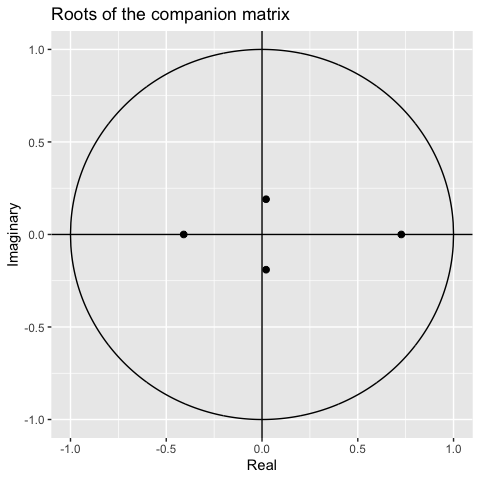
\includegraphics{12-exportedfigures/stability.plot-1} \end{center}
\vspace{-3mm}
\label{graf:stability}
\fonte{Desenvolvido a partir de dados coletados}
\vspace{-2mm}
\end{grafico}

\begin{center}\rule{0.5\linewidth}{0.5pt}\end{center}

\begin{center}\rule{0.5\linewidth}{0.5pt}\end{center}

\printbibliography[title=\hspace{45pt}{REFERÊNCIAS}]

\end{document}
